\documentclass{tufte-handout}

\usepackage{amssymb,amsmath}
% \usepackage{mathspec}
\usepackage{graphicx,grffile}
\usepackage{longtable}
\usepackage{booktabs}

\newtheorem{mydef}{Definition}[section]
\newtheorem{thm}{Theorem}[section]
\setcounter{section}{6}

\DeclareMathOperator*{\argmin}{arg\,min}
\DeclareMathOperator*{\argmax}{arg\,max}
\newcommand{\Lim}[1]{\raisebox{0.5ex}{\scalebox{0.8}{$\displaystyle \lim_{#1}\;$}}}
\newcommand{\E}{\mathbb{E}}
\newcommand{\Prob}{\mathbb{P}}
\newcommand{\V}{\text{Var}}
\newcommand{\iid}{\stackrel{iid}{\sim}}
\newcommand{\cblack}{\color{Black}}
\newcommand{\cblue}{\color{MidnightBlue}}

\providecommand{\tightlist}{%
  \setlength{\itemsep}{0pt}\setlength{\parskip}{0pt}}

\begin{document}

\justify

{\LARGE Handout 08: Multiple Comparisons Problem}

\vspace*{18pt}

\noindent
The results we have established for hypothesis testing concern a
single, specific test. Things become more complex when looking at
multiple tests all at once. Consider for example running hypothesis
tests from $100$ experiments with a significant level of $0.95$. Even
if the null hypothesis is in fact true in each experiement, if we
cherry-pick the lowest p-value, we would expect on average to have
$5$ of the tests erroneously show up as significant. Let's see some
approaches to addressing this.

Consider a sequence of $m$ null hypothesis $H_1, \ldots, H_m$ and the
corresponding p-values defined by $p_1, \ldots, p_m$. The probability
of incorrectly rejecting at least one of the hypotheses is called the
\textbf{family-wise error rate (FWER)}.\footnote{
  There are other less conservative ways of controlling the error rates that
  arise when doing testing of many procedures. These control other quantities,
  usually something such as the \textbf{false discovery rate (FDR)}. We will
  not cover these directly this semester, but it would be a good project topic
  for the final project if you are interested.
}
Assume that all of the null
hypothesis are in fact true; what is the probability that we incorrectly
reject one of them using a cut-off significance level of $\alpha$? Well,
we have that:
\begin{align*}
\text{FWER} = \Prob \left[ \bigcup_{j=1}^m \left\{ p_j \leq \alpha \right\} \right]
&\leq \sum_{j=1}^m \Prob \left[ p_j \leq \alpha \right] = \sum_{j=1}^m \alpha = m \cdot \alpha.
\end{align*} 
So the probability of making at least one mistake could be as high as
$m$ times the confidence level. This means that if we actually want an
error rate of $\alpha$, we need to consider a cut-off value $m$ times
smaller than this error rate. Alternatively, we could adjust the p-values
by multiplying them by the number of tests. That is, consider $p_j' = p_k \cdot m$.
This gives:
\begin{align*}
\text{FWER} = \Prob \left[ \bigcup_{j=1}^m \left\{ p_j' \leq \alpha \right\} \right]
&\leq \sum_{j=1}^m \Prob \left[ p_j \cdot m \leq \alpha \right] =
\sum_{j=1}^m \frac{\alpha}{m} = \alpha.
\end{align*} 
Adjusting the p-values tends to be a better choice because they can be
presented on their own terms without having to also specify the adjustment.

The above procedure shows that we will control the FWER if all of the
hypotheses are true. What happens when only $k < m$ of the null hypotheses
are in fact true? It turns out in this case the same equation above holds,
but with the intersection taken over only the $k$ true null hypothesis. Our
correction will be valid, though overly conservative. So, the p-value adjustment
provides valid control over the FWER.\footnote{
  Note that by the error rate we refer only to what some sources call the
  `Type I' error, falsely rejecting the null hypothesis. Controlling the 
  the power of the test to detect false null-hypothesis depends on the
  specific structure of the data and sampling that we do not have access 
  to in this setup.
} The procedure outlined here is called the \textbf{Bonferroni correction}.
There is a slightly stronger and equally valid version called the
\textbf{Holm-Bonferroni correction} that we will see on today's worksheet.
This procedure should be used to adjust p-values whenever you are running
a large number of tests and want to be able to reliably trust any of the
individual findings in isolation.

\newpage

\begin{center}
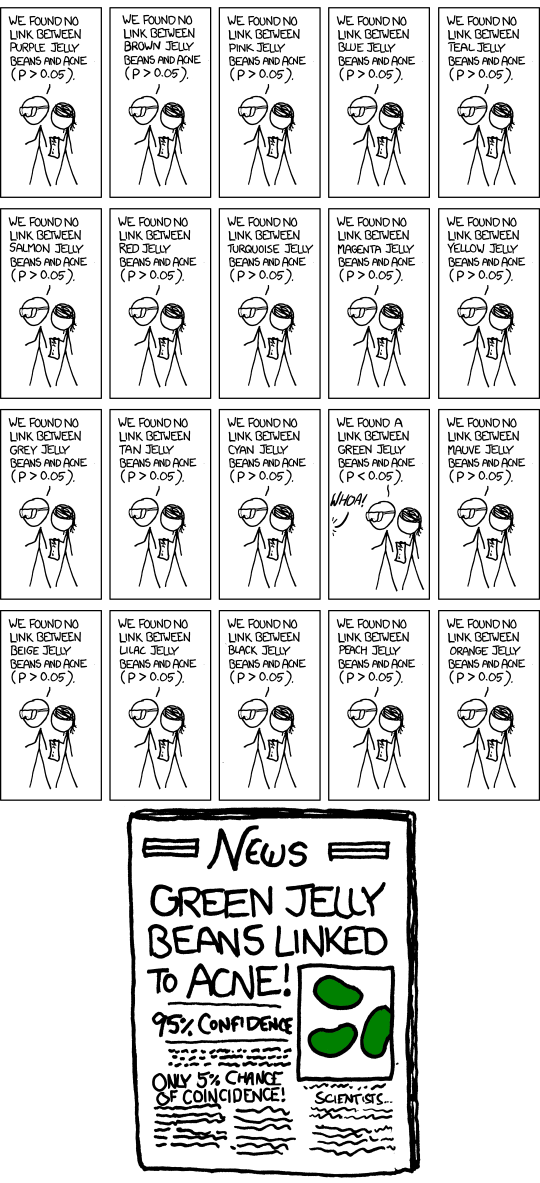
\includegraphics[width=0.85\textwidth]{../extra/significant.png} \\
\footnotesize{CC-BY NC 2.5, Randall Munroe, \texttt{xkcd.com}}
\end{center}


\end{document}

